\documentclass[border=10pt]{standalone}
\usepackage{amsmath}
\usepackage{tikz}
\usetikzlibrary{arrows.meta,calc}
\definecolor{acc}{HTML}{0D9488}
\definecolor{ink}{HTML}{1A1D21}
\definecolor{mut}{HTML}{646A72}
\begin{document}
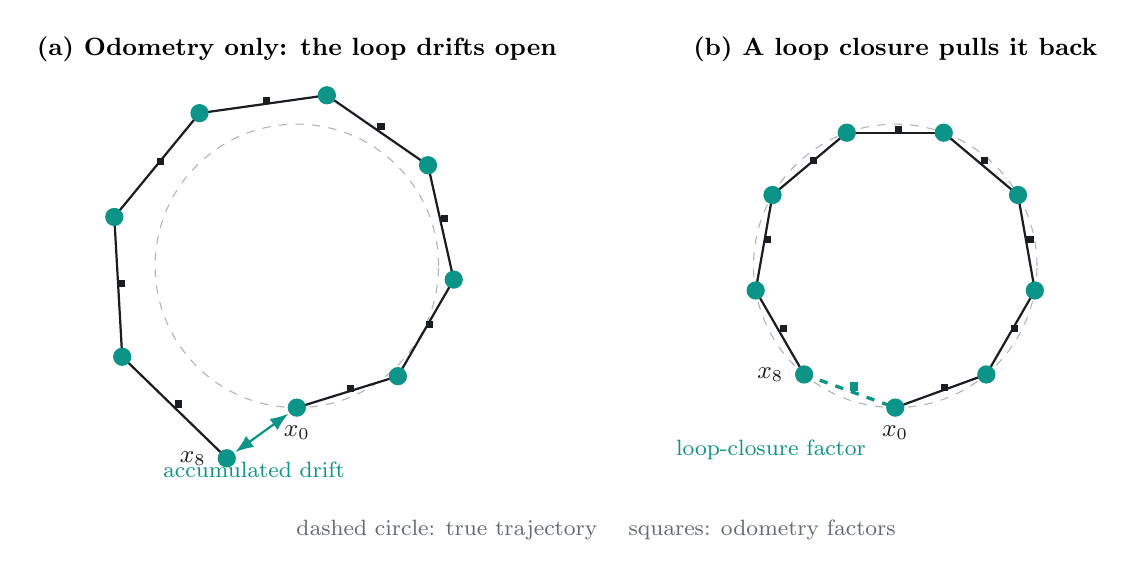
\begin{tikzpicture}[>=Latex, font=\small]
  \foreach \panel/\drift/\title in {0/1/{(a) Odometry only: the loop drifts open}, 7.6/0/{(b) A loop closure pulls it back}} {
    \begin{scope}[xshift=\panel cm]
      \node[font=\bfseries\small] at (0,2.75) {\title};
      \draw[mut!50, dashed] (0,0) circle (1.8);
      \foreach \k in {0,...,8} {
        \pgfmathsetmacro{\ang}{-90 + 40*\k + \drift*2.5*\k}
        \pgfmathsetmacro{\rad}{1.8 + \drift*0.1*\k}
        \coordinate (x\k) at (\ang:\rad);
      }
      \foreach \k [evaluate=\k as \j using int(\k+1)] in {0,...,7} {
        \draw[ink, thick] (x\k) -- (x\j);
        \fill[ink] ($(x\k)!0.5!(x\j)$) rectangle +(0.09,0.09);
      }
      \foreach \k in {0,...,8} {
        \fill[acc] (x\k) circle (3.3pt);
      }
      \node[below=3pt, text=ink] at (x0) {$x_0$};
      \node[left=4pt, text=ink] at (x8) {$x_8$};
      \ifnum\drift=0
        \draw[acc, very thick, dashed] (x8) -- (x0);
        \fill[acc] ($(x8)!0.5!(x0)$) rectangle +(0.11,0.11);
        \node[text=acc, font=\footnotesize, anchor=north] at ($(x8)!0.5!(x0)+(-1.0,-0.5)$) {loop-closure factor};
      \else
        \draw[<->, acc, thick] ($(x8)!0.12!(x0)$) -- ($(x8)!0.88!(x0)$);
        \node[text=acc, font=\footnotesize, anchor=north] at ($(x8)!0.5!(x0)+(-0.1,-0.25)$) {accumulated drift};
      \fi
    \end{scope}
  }
  \node[text=mut, font=\footnotesize] at (3.8,-3.35) {dashed circle: true trajectory \quad squares: odometry factors};
\end{tikzpicture}
\end{document}
